\subsection{Postać stałej podwójnej precyzji. Podać przykłady}
\begin{lstlisting}[language=Fortran, caption=dyrektywa implicit]
double precision :: foo !3.54D0, 35.4D-1
\end{lstlisting}

\subsection{Na czym polega reguła pierwszej litery}
\label{sec:lit}
Jeśli zmienna nie zostanie zadeklarowana to Fortran77 przyjmie
regułę pierwszej litery w nazwie.
\begin{itemize}
\item Zmienna o nazwie zaczynające się od i, j, k, l, m, n zostaje
automatycznie przypisana do typu INTEGER
\item pozostałe do typu REAL.
\end{itemize}

\subsection{Podać przykład zastosowania dyrektywy IMPLICIT}
\begin{lstlisting}[language=Fortran, caption=dyrektywa implicit]
program test
	implicit none
	integer :: a, b, c
	...
end program
\end{lstlisting}
\subsection{Co musi wystąpić po dyrektywie IMPLICIT NONE?}
Deklaracja stałych (anuluje regułę pierwszej litery (\ref{sec:lit}))
\subsection{Sposoby deklaracji wymiaru i rozmiaru tablicy (zmiennej indeksowanej). Jaki jest maksymalny wymiar tablicy?}
Maksymalny 7-wymiarowa tablica.\\
\begin{itemize}
\item \textbf{TYP <nazwa> DIMENSION <nazwa>(n1:m1,n2:m2)}
\item \textbf{TYP <nazwa>(n1:m1,n2:m2)}
\end{itemize}


\subsection{Jaka jest różnica między funkcjami wewnętrznymi ATAN i ATAN2?}
\begin{itemize}
\item ATAN(x) - arctg w radianach
\item ATAN2(x,y) - x,y-wspł. wektora, wynik w radianach
\end{itemize}
\subsection{Wymień operatory arytmetyczne i kolejność ich wykonywania}
Zgodnie z priorytetem(jeśli równoważne to od prawej strony):
\begin{itemize}
\item potęgowanie "A**B"
\item mnożenie "A*B", dzielenie "A/B"
\item dodawanie, odejmowanie
\end{itemize}
\subsection{Wymień operatory relacji}
\begin{itemize}
\item .LT.
\item .LE.
\item .EQ.
\item .NE.
\item .GE.
\item .GT.
\end{itemize}
\subsection{Wymień operatory logiczne}
\begin{itemize}
\item .NOT.
\item .AND.
\item .OR.
\item .EQV.
\item .EQV. rownoważność
\item .NEQV.
\end{itemize}
\begin{figure}[h!]
\centering
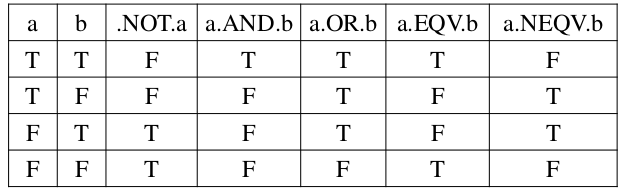
\includegraphics[scale=0.4]{oplog}
\end{figure}
\subsection{Podaj typ wyniku i jego wartość: 2/4, 2./4, 2d0/4, 5/2, 2./5}
2/4=0, 2./4=0.500000000, d20/4=0.50000000000000000, 5/2=2, 2.5=0.400000006


\subsection{Podaj postać bezwarunkowej instrukcji skoku}
\textbf{GO TO <etykieta>}
\begin{lstlisting}[language=Fortran, caption=cos]
10	n = n + 1
	go to 10
\end{lstlisting}

\subsection{Podaj postać instrukcji warunkowej prostej}
IF (wyrazenie logicze) instrukcja
\begin{lstlisting}[language=Fortran, caption=cos]
	if (foo.LE.2) bar=2
\end{lstlisting}

\subsection{Podaj postać blokowej instrukcji warunkowej}

\begin{lstlisting}[language=Fortran, caption=cos]
IF ( wyrazenie logiczne ) THEN
...
...
END IF
\end{lstlisting}

\subsection{Podaj postać instrukcji warunkowej złożonej}

\begin{lstlisting}[language=Fortran, caption=cos]
IF ( wyrazenie logiczne ) THEN
...
ELSE IF (warunek) THEN
...
ELSE
...
END IF
\end{lstlisting}

\subsection{Podaj postać arytmetycznej instrukcji warunkowej}

\begin{lstlisting}[language=Fortran, caption=cos]

\end{lstlisting}

\subsection{Podaj postać instrukcji cyklu}

\begin{lstlisting}[language=Fortran, caption=cos]
DO iterator=start, stop, step
...
...
END DO 
\end{lstlisting}

\subsection{Co to jest urządzenie standardowe? Podaj postać instrukcji czytania danych z urządzenia standardowego}
urzadzenie wejscia-wyjscia umozliwiające komunikację między programem a srodowiskiem zewnętrznym(dysk, ekran ...)

\begin{lstlisting}[language=Fortran, caption=cos]
open(10, file="cache.txt", status="old")
read(10,*) foo
close(10)
\end{lstlisting}

\subsection{Podaj postać instrukcji pisania wartości tablicy jednowymiarowej z wykorzystaniem listy cyklu (DO implikowanego)}
\begin{lstlisting}[language=Fortran, caption=cos]
program X
dimension T(3)
do j=1,3
  T(j) = float(j**2)
  write(*,*) T(j)
  do i=1,2
    
end do
end program
\end{lstlisting}

